\chapter{The Sunayev-Zeldovich Effect}
*** NEED SOURCES FOR ATOMIC PHYSICS OF \sze ***
\section{Atomic Physics}
The thermal \sze is one possible tracer. \sze refers to the inverse compton scattering of CMB photons off of hot electrons in the WHIM. 

Compton Scattering is a form of inelastic scattering between light and free charged particles, such as electrons. There is a momentum transfer between the photon in the interaction, and the charged particle, and so the photon's wavelength changes as a result of the scattering. 

\begin{figure}
\centering
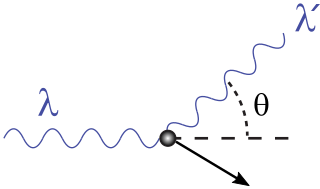
\includegraphics[scale=0.5]{/home/mitchell/Documents/masters/masters/thesis/Ver_2/figures/320px-Compton-scattering.png}
\label{fig:compton_scattering}
\caption{Compton Scattering}
\end{figure}


It was first described in the context of X-rays interacting with electrons in atoms, and so regular Compton Scattering is taken to describe the interaction between a high energy photon, and a low energy particle (or one at rest). By applying principles of conservation of momentum, and conservation of energy,  the formula for the shift in wavelength as a result of this scattering is given by
\begin{equation}
	\Delta \lambda = \frac{h}{m_ec}\left(1-\cos\theta\right)
	\label{eqn:compton_shift}
\end{equation}
where $m_e$ is the mass of the electron, and $\theta$ is the angle between the incident and scattered trajectories.

For the \sze however, the energies of the photons in question are much lower than the energies of the electrons involved, so the frequency shift is parametrised by something called the Compton $y$-parameter. The full expression for the Compton $y$-parameter is 
\begin{equation}
y = \int \frac{k_B T_e}{m_e c^2} n_e \sigma_T d\mathcal{l}
\label{eqn:y_param}
\end{equation}
where $m_e c^2$, $k_B$, and $\sigma_T$ are the electron rest mass energy, Boltzmann constant, and Thompson Cross Section respectively. These are all well defined constants, and so have no effect on the integration. The $y$-parameter therefore amounts to the line-of-sight integration over $n_e T_e$, which are the electron gas density and temperature. The degeneracy between temperature and pressure can be broken in principle by obtaining measurements of one of the two quanties, which we in princple take from hydrodynamical simulations.

\section{CMB Signal}


Given the signal-to-noise ratio expected for the thermal \sze of a single filament, many such filaments must be co-added, so as to drive the signal-to-noise to a detectable level. Initially outlined in \cite{2016MNRAS.457.2391C} for application to weak gravitational lensing maps, it was found that stacking \~ 135 000 pairs yielded a filament mass at \~ 4.5 $\sigma$ confidence. Further follow up using the Canada France Hawaii Telescope Lensing Survey (CFHTLenS), and the Sloan Digital Sky Survey's (SDSS) Luminous Red Galaxy (LRG) catalogue by \cite{2017MNRAS.468.2605E} detected the weak lensing signal from stacked filaments at 5$\sigma$ confidence.

Investigations by \cite{2014PhRvD..89b3508V}, \cite{2015JCAP...09..046M}, and \cite{2015JCAP...10..047H} established firmly that there is a correlation between weak gravitational lensing from CFHTLenS and tSZ signals from \planck , which suggests that we can use tSZ in the same way as weak lensing, without having to be careful about the peculiarities assosciated with weak lensing, such as sufficiently nulling spherical components. This was further reinforced by \cite{2014JCAP...02..030H}, who reported a $6.2 \sigma$ correlation between the \planck  lensing potential and the \planck  tSZ map. 
